% One path of length 8 that first hits height 2 at time 2, and the path
% obtained by reflecting only the initial segment across that height.
% Original heights: 0,1,2,3,2,1,2,1,2.
% Reflected:       4,3,2,3,2,1,2,1,2.
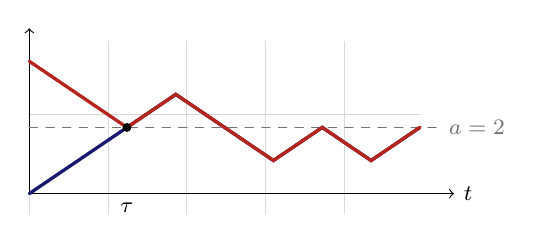
\begin{tikzpicture}[x=0.62cm,y=0.42cm,line cap=round]
  \draw[black!15] (0,-0.6) grid (8,4.6);
  \draw[->] (0,0)--(8.7,0) node[right,font=\footnotesize] {$t$};
  \draw[->] (0,0)--(0,5);
  \draw[dashed,black!55] (0,2)--(8.4,2) node[right,font=\footnotesize] {$a=2$};
  \draw[MidnightBlue,very thick] (0,0)--(1,1)--(2,2)--(3,3)--(4,2)--(5,1)--(6,2)--(7,1)--(8,2);
  \draw[BrickRed,very thick] (0,4)--(1,3)--(2,2)--(3,3)--(4,2)--(5,1)--(6,2)--(7,1)--(8,2);
  \fill (2,2) circle (1.6pt);
  \node[font=\footnotesize,below] at (2,0) {$\tau$};
\end{tikzpicture}
